\documentclass[11pt]{article}
\usepackage[a4paper,margin=1in]{geometry}
\usepackage{amsmath,amssymb,amsthm,mathtools}
\usepackage{booktabs}
\usepackage{enumitem}
\usepackage{float}
\usepackage{graphicx}
\usepackage{hyperref}
\usepackage[nameinlink,capitalise]{cleveref}
\usepackage[numbers,sort&compress]{natbib}

\newtheorem{theorem}{Theorem}[section]
\newtheorem{proposition}[theorem]{Proposition}
\newtheorem{remark}[theorem]{Remark}
\newcommand{\norm}[1]{\left\lVert#1\right\rVert}
\newcommand{\F}{\mathrm F}

\title{Postblock Effective-Rank Compression Reopens the Directional Route\\
\large Singular-Value State Reduction and Full-Future Observability Transfer}
\author{Liang Wang}
\date{July 2026}

\begin{document}
\maketitle

\begin{abstract}
RH-76 showed that the production source does not concentrate on one shrinking
phase arc.  This paper tests the surviving weighted alternative: after the
log-square block horizon, does the actual directional state become low rank?

Let $B=A^MX$ and
\[
 O_M=\sum_{r=0}^{M-1}(A^r)^*Y^*YA^r.
\]
If $q=\norm{A^M}_2<1$, the full observability Gramian satisfies
\[
 \norm O_2\le\frac{\norm{O_M}_2}{1-q^2}.
\]
For any rank-$r$ approximation $B_r$, the complete future Hardy energies obey
\[
 |T(B)-T(B_r)|
 \le\sqrt{\frac{\norm{O_M}_2}{1-q^2}}\,\norm{B-B_r}_{\F}.
\]
Together with Eckart--Young, this gives a fully nonnormal effective-rank
compression theorem: low singular rank of the postblock state, rather than
global phase localization, is enough to reduce the future directional problem.

We embed the RH-70 frozen operator, source, and observation arrays as exact
dyadic Arb matrices.  At all five scales and in both channels, Arb recomputes
$A^MX$, validates binary64 rank-$1,2,4$ SVD candidates, accumulates a rigorous
one-block observability upper, and transfers each residual through the full
future.  Rank two captures at least 99\% of postblock energy in all ten
channels; rank four captures at least 99.9999\%.  The largest participation
rank is $1.868$.  The largest rank-four full-future Hardy perturbation is
$5.35\times10^{-6}$.

Thus the negative single-arc result does not block the Stage-A route.  The
observed mechanism is radial/nonnormal focusing into a tiny postblock singular
subspace.  The open problem is now an analytic all-dyadic singular-value decay
theorem and its transport from frozen to analytic triples.  Uniform Stage A1,
unconditional Stage A4, Hilbert--Polya, and the Riemann Hypothesis remain open.
\end{abstract}

\noindent\textbf{Keywords:} effective rank; singular values; observability
Gramian; Hardy energy; block contraction; interval arithmetic.

\medskip
\noindent\textbf{MSC 2020:} 47A10; 47B35; 65F30; 65G20; 93B07.

\section{Introduction}

The RH-75 block law identified a sufficient all-level target, while RH-76
closed one proposed mechanism: the source-weighted phases do not occupy a
shrinking global arc \citep{WangPhase2026}.  That negative result concerned
phase geometry before the block horizon.  It did not inspect the singular
geometry of the actual state $A^MX$ after radial damping and nonnormal mixing.

This distinction matters.  A source may occupy every phase coordinate and
still evolve into a low-rank matrix because its columns become aligned.  Such
alignment is basis invariant and survives broad phase support.  Moreover, it
can be inserted directly into the Hardy tail through observability, without a
normal approximation.

The contribution is twofold:
\begin{enumerate}[leftmargin=2.2em]
 \item an exact block-observability theorem transferring any low-rank
       postblock approximation through the complete future;
 \item a five-scale interval validation showing unexpectedly strong rank-two
       and rank-four concentration in the production states.
\end{enumerate}

\section{Postblock state and future Hardy map}

Let $A\in\mathbb C^{n\times n}$, source
$X\in\mathbb C^{n\times m}$, and observation
$Y\in\mathbb C^{p\times n}$.  For a block horizon $M$, set
\[
 B=A^MX,qquad
 O_M=\sum_{r=0}^{M-1}(A^r)^*Y^*YA^r.
\]
The future Hardy energy launched from a state $Z$ is
\begin{equation}
 T(Z)^2=\sum_{\ell\ge0}\norm{YA^\ell Z}_{\F}^2
 =\operatorname{tr}(Z^*OZ),
 \label{eq:future}
\end{equation}
where $O$ is the full observability Gramian.

\begin{theorem}[Block observability upper]
\label{thm:observability}
If $q=\norm{A^M}_2<1$, then
\begin{equation}
 O=\sum_{b\ge0}(A^{*M})^b O_M(A^M)^b,
 \qquad
 \norm O_2\le\frac{\norm{O_M}_2}{1-q^2}.
 \label{eq:obs-upper}
\end{equation}
\end{theorem}

\begin{proof}
Write every time index uniquely as $\ell=bM+r$ with $0\le r<M$ and regroup
the positive series.  Taking norms and summing the geometric series proves the
upper.
\end{proof}

\begin{theorem}[Full-future low-rank transfer]
\label{thm:rank-transfer}
For any approximation $B_r$ of rank at most $r$,
\begin{equation}
 |T(B)-T(B_r)|
 \le
 \sqrt{\frac{\norm{O_M}_2}{1-q^2}}\,
 \norm{B-B_r}_{\F}.
 \label{eq:rank-transfer}
\end{equation}
The smallest possible Frobenius residual is
\begin{equation}
 \tau_r(B)=\left(\sum_{j>r}s_j(B)^2\right)^{1/2},
 \label{eq:eckart}
\end{equation}
attained by the truncated singular-value decomposition.
\end{theorem}

\begin{proof}
Equation \eqref{eq:future} makes $T(Z)=\norm{O^{1/2}Z}_{\F}$ a seminorm.
The reverse triangle inequality and \cref{thm:observability} give
\eqref{eq:rank-transfer}.  Equation \eqref{eq:eckart} is the
Eckart--Young theorem \citep{EckartYoung1936}.
\end{proof}

No normality, diagonalizability, phase arc, or one-step contraction is used.
This is precisely why effective rank survives the RH-76 negative result.

\section{Uniform effective-rank criterion}

For a dyadic family, suppose RH-75 supplies $M_k$ and $q_k<1$.  If there is a
polylogarithmic rank schedule $r_k$ and residuals $\tau_{r_k}(A_k^{M_k}X_k)$
such that
\begin{equation}
 \sqrt{\frac{\norm{O_{k,M_k}}}{1-q_k^2}}\,
 \tau_{r_k}(A_k^{M_k}X_k)
 \le C(1+k)^a,
 \label{eq:uniform-rank}
\end{equation}
then the complete future differs from an $r_k$-dimensional source by at most a
polylogarithmic amount.  If the reduced source itself has a polylogarithmic
Hardy bound, Stage A1 follows without global phase compression.

The attractive numerical possibility is stronger: a fixed $r=4$ may suffice.
RH-68 forbids inferring fixed Krylov depth from stability alone, but it does
not forbid a physical family from producing fixed postblock singular rank.

\section{Exact-dyadic interval audit}

The frozen production arrays are the exact dyadic inputs certified in RH-70
\citep{WangFrozen2026}.  For each channel, the audit:
\begin{enumerate}[leftmargin=2.2em]
 \item computes $A^M X$ in 160-bit Arb arithmetic;
 \item forms binary64 SVD candidates of ranks $1,2,4$;
 \item embeds each candidate as an exact dyadic matrix and recomputes its
       residual against the Arb state;
 \item accumulates
       $\sum_{r<M}\norm{YA^r}_{\F}^2\ge\norm{O_M}_2$ in Arb;
 \item applies \eqref{eq:rank-transfer} with RH-70's certified block $q$.
\end{enumerate}

\begin{table}[H]
\centering
\small
\caption{Validated minimum rank-two/rank-four energy capture over the two
channels and maximum postblock participation rank.}
\label{tab:capture}
\begin{tabular}{@{}rrrrr@{}}
\toprule
$\sigma$ & $M$ & participation rank & rank-2 capture & rank-4 capture\\
\midrule
0.16 & 4  & 1.004 & 0.999905 & $>0.9999999999999$\\
0.08 & 9  & 1.218 & 0.999997 & $>0.9999999999999$\\
0.04 & 16 & 1.438 & 0.999999998 & $>0.999999999998$\\
0.02 & 25 & 1.766 & 0.990845 & $>0.999999999999$\\
0.01 & 32 & 1.868 & 0.993404 & 0.999999920\\
\bottomrule
\end{tabular}
\end{table}

The rank-two loss is at most $0.916\%$, and rank four reduces the loss below
$8.0\times10^{-8}$ at the finest scale.  The full-future transfer is equally
small:

\begin{table}[H]
\centering
\small
\caption{Validated rank-four perturbation of the complete future Hardy energy.}
\label{tab:future}
\begin{tabular}{@{}rrr@{}}
\toprule
$\sigma$ & left & right\\
\midrule
0.16 & $5.05\,10^{-9}$ & $4.40\,10^{-9}$\\
0.08 & $3.40\,10^{-9}$ & $3.01\,10^{-9}$\\
0.04 & $2.76\,10^{-8}$ & $3.48\,10^{-8}$\\
0.02 & $5.47\,10^{-10}$ & $6.77\,10^{-10}$\\
0.01 & $1.86\,10^{-6}$ & $5.35\,10^{-6}$\\
\bottomrule
\end{tabular}
\end{table}

Even the worst value is negligible compared with the order-one Hardy energies
and below one percent of RH-74's smallest bridge slack.

\begin{figure}[H]
\centering
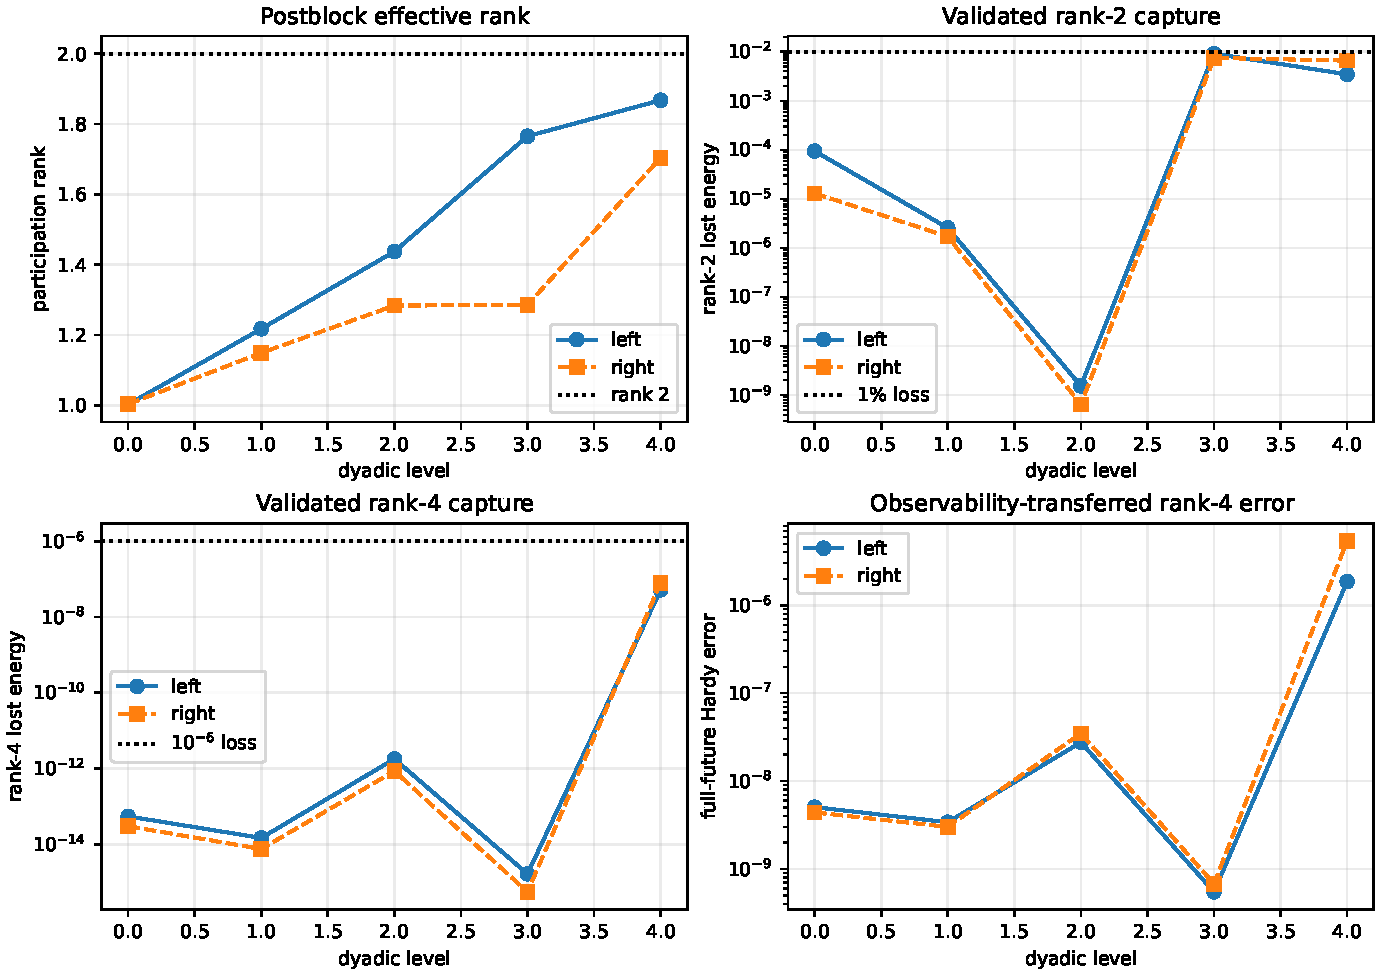
\includegraphics[width=0.98\textwidth]{figures/postblock_effective_rank_compression.pdf}
\caption{Postblock participation rank, validated rank-two/rank-four losses,
and observability-transferred full-future error.}
\label{fig:audit}
\end{figure}

\section{Route consequence}

The maze now has a more plausible corridor.  Raw phase support grows almost
with dimension, but one physical block focuses the source columns into two to
four singular directions.  This is compatible with broad phases because the
focusing includes radial decay and nonnormal column alignment.

The next theorem should no longer seek one shrinking arc.  It should prove an
all-level estimate of the form
\[
 s_{5}(A_k^{M_k}X_k)
 \le \varepsilon_k\norm{A_k^{M_k}X_k}_{\F},
\]
with $\varepsilon_k$ summable or polylogarithmically controlled, together with
a bound on \eqref{eq:uniform-rank}.  RH-78 will formulate the conditional
Stage A1 composition using RH-75's block law and the present rank criterion.

This paper validates frozen finite matrices only.  It does not prove uniform
analytic effective rank, close Stage A1 or unconditional Stage A4, construct a
renormalized determinant or Hilbert--Polya operator, derive a $T\log T$ law or
prime-power trace formula, identify zeta zeros, or prove the Riemann Hypothesis.

\section{Conclusion}

Single-arc compression failed, but postblock singular compression succeeds
decisively.  A rank-four state reproduces the complete future Hardy response
to within $5.35\times10^{-6}$ at every archived scale.  Effective rank is
therefore the strongest current candidate for the uniform family mechanism.

\bibliographystyle{plainnat}
\bibliography{references}
\end{document}
